\section{Kinematika}
\paragraph{Enakomerno pospešeno gibanje} (\(\ds a := \frac{dv}{dt} = \text{const}\)).
%
\begin{itemize}
    \item \(\ds dv = a \, dt \lthen \int_{v_0}^{v} \, dv = a \int_{0}^{t} \, dt \lthen v - v_0 = at \lthen  \boxed{v = v_0 + at}\)
    \item \(\ds v := \frac{ds}{dt} \lthen ds = (v_0 + at) \, dt \lthen \int_{0}^{s} \, ds = \int_{0}^{t} (v_0 + at) \, dt \lthen \boxed{s = v_0t + \frac{1}{2}at^2}\)
    \item \(\ds v = \frac{ds}{dt}, \ a = \frac{dv}{dt} \lthen v \, dt = ds, \ a \, dt = dv \lthen \frac{v}{a} = \frac{ds}{dv} \lthen v \, dv = a \, ds \lthen \int_{v_0}^{v} v \, dv = \int_{0}^{s} a \, ds\)
    
    \(\ds \lthen \frac{v^2}{2} - \frac{v_0^2}{2} = as \lthen \boxed{v^2 - v_0^2 = 2as}\) (če imamo delo z pojemkom, spremenimo predznak)
    \item \textbf{Enakomerno gibanje:} Vzemimo \(a = 0\)
\end{itemize}
%
\paragraph{Prosti pad} (\(v_0 = 0, \  g = 9.8 \  \text{m} / \text{s}^2\)).
\begin{itemize}
    \item \(\ds \boxed{v = gt, \ t = \sqrt{\frac{2h}{g}}, \ h = \frac{1}{2} g t^2}\)
\end{itemize}

\paragraph{Relativna hitrost:} \(\vec{v}_r = \vec{v}_1 - \vec{v}_2, \ v_r = |\vec{v}_1 - \vec{v}_2|\)
%

\paragraph{Vodoravni met}
\ 

\begin{minipage}[t]{0.35\textwidth}
    \vspace{0pt}
  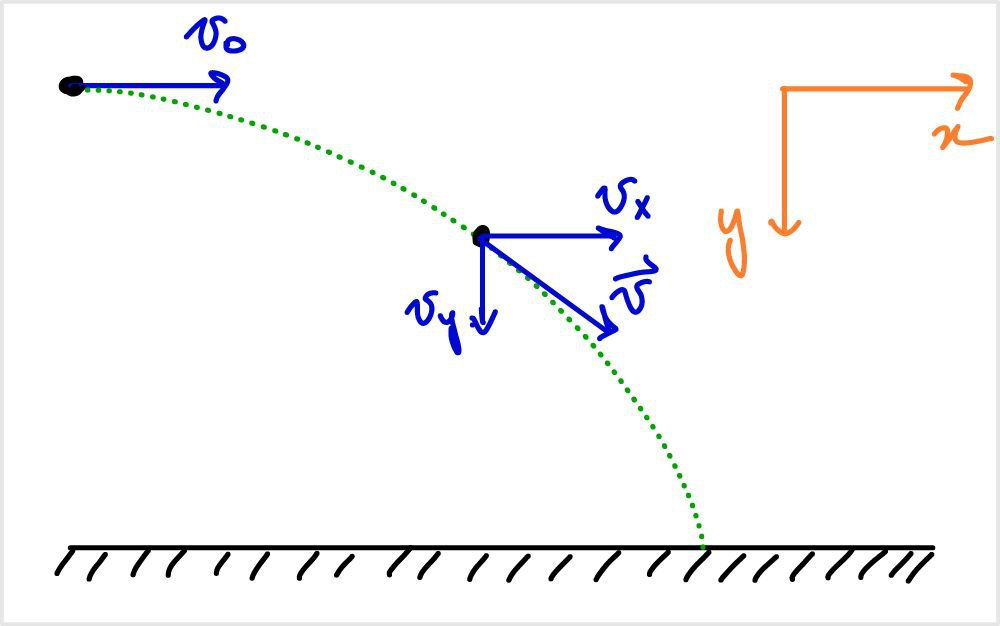
\includegraphics[width=\linewidth]{img/01_001.jpg} 
\end{minipage}
\hfill
\begin{minipage}[t]{0.60\textwidth}
    \vspace{0pt}
    \begin{itemize}
        \item \(x(t) = v_0 t, \ y(t) = \frac{1}{2}gt^2\)
        \item \(v_x = v_0 = \text{const}, \ v_y(t) = gt\)
    \end{itemize}
\end{minipage}
%
\paragraph{Poševni met}
\ 

\begin{minipage}[t]{0.35\textwidth}
    \vspace{0pt}
  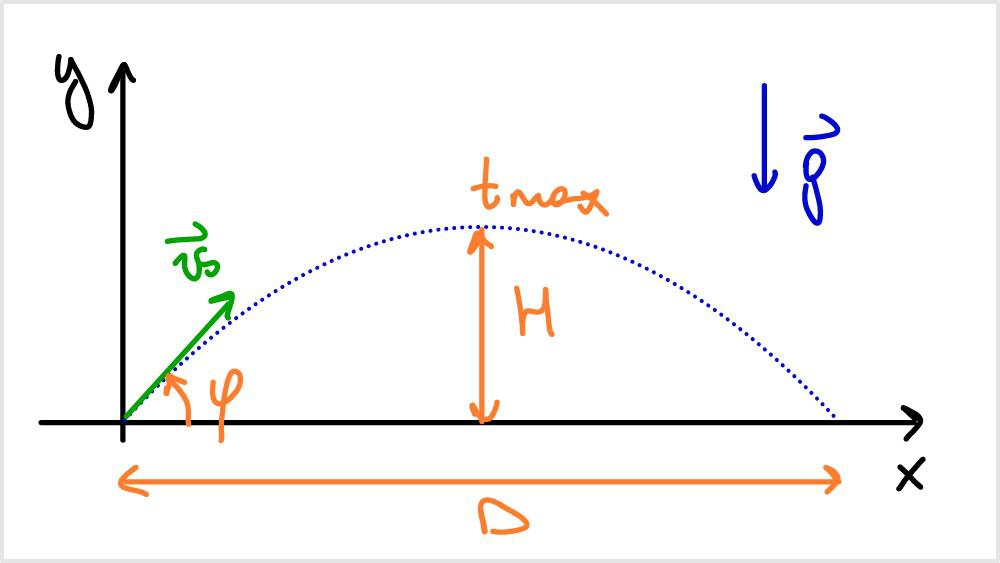
\includegraphics[width=\linewidth]{img/01_002.jpg} 
\end{minipage}
\hfill
\begin{minipage}[t]{0.60\textwidth}
    \vspace{0pt}
    \begin{itemize}
        \item \(x(t) = v_0 t \cos \phi, \ y(t) = v_0 t \sin \phi - \frac{1}{2}gt^2\)
        \item \(v_x = v_0 \cos \phi, \ v_y(t) = v_0 \sin \phi - gt\)
        \item \(\boxed{t_\text{max} = \frac{v_0 \sin \phi}{g}, \ D = \frac{v_0^2 \sin 2 \phi}{g}, \ H = \frac{v_0^2\sin^2 \phi}{2g}}\)
        \item Gibanje lahko razdelimo na dva dela: do \(H_\text{max}\) (poševni met) in po \(H_\text{max}\) (vodoravni met)
        \item Vodoravni met je posebni primer poševnega meta pri \(\phi = 0\)
    \end{itemize}
\end{minipage}
%
\paragraph{Kroženje}
\ 

\begin{minipage}[t]{0.25\textwidth}
    \vspace{0pt}
  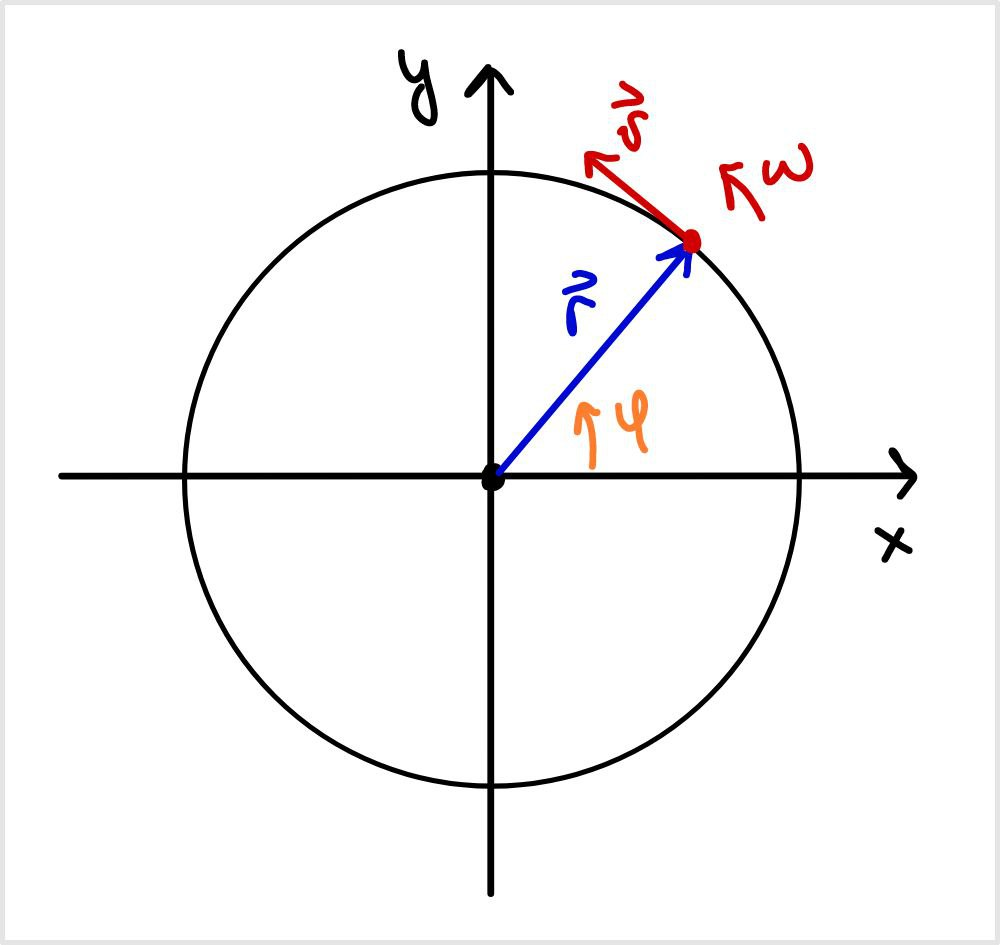
\includegraphics[width=\linewidth]{img/01_003.jpg} 
\end{minipage}
\hfill
\begin{minipage}[t]{0.70\textwidth}
    \vspace{0pt}
    \begin{itemize}
        \item \(\vec{r}(t) = r (\cos \phi, \sin \phi), \ \vec{v}(t) = r \omega (-\sin \phi, \cos \phi)\), kjer \(\omega = \dot{\phi}\) \df{kotna hitrost}
        \begin{itemize}
            \item \(s = r \phi\), če merimo \(\phi\) v radianih
        \end{itemize}
        \item \(a(t) = r \alpha (-\sin \phi, \cos \phi) + r \omega^2 (-\cos \phi, -\sin \phi)\), kjer \(\alpha = \ddot{\phi}\) \df{kotni pospešek}
        \begin{itemize}
            \item \(\vec{a}_t = r \alpha (-\sin \phi, \cos \phi)\) je tangentni pospešek (spreminjanje velikosti \(\vec{v}\))    
            \item \(\vec{a}_r = r \omega^2 (-\cos \phi, -\sin \phi)\) je radialni pospešek (spreminjanje smeri \(\vec{v}\))        
        \end{itemize}
        \item \(\ds \boxed{v = r \omega,\ a_t = r \alpha, \ a_r = r \omega^2 = \frac{v^2}{r}, \ a = \sqrt{a_r^2 + a_t^2}}\)
        \item \(\ds \omega = 2 \pi \nu, \ \nu = \frac{1}{t_0}\), kjer \(t_0\) je čas enega obrata, \(\nu\) je \df{frekvenca}
        \item Enakomerno pospešeno kroženje ima iste enačbe kot enakomerno pospešeno gibanje
    \end{itemize}
\end{minipage}

\paragraph{Vektorski opis kroženja}
\begin{itemize}
    \item Definiramo \(\vec{\phi} = (0, 0, \phi)\) (smer \(\vec{\phi}\) lahko dobimo po pravilu desnega vijaka), potem
    \begin{itemize}
        \item \(\vec{v} = \vec{\omega} \times \vec{r}\)
        \item \(\vec{a} = \vec{\alpha} \times \vec{r} + \vec{\omega} \times (\vec{\omega} \times \vec{r})\)
    \end{itemize}
\end{itemize}

\paragraph{Splošno gibanje}
\begin{itemize}
    \item \(\ds R = \frac{v^2}{a_r}, \ \omega = \frac{a_r}{v}, \ \alpha = \frac{a_t a_r}{v^2}\) (vsako gibanje je trenutno kroženje), \(a_t, a_r\) sta komponenti \(g\)
\end{itemize}

\paragraph{Splošni nasveti}
\begin{itemize}
    \item Lahko obrnemo čas (začetek = konec)!
\end{itemize}

\section{Dinamika}
\paragraph{Newtonovi zakoni}
\begin{enumerate}
    \item \(\sum \vec{F} = 0 \lthen \vec{v} = \text{const}\)
    \item \(\sum \vec{F} = m \vec{a}\) 
    \item \(\vec{F}_{12} = -\vec{F}_{21}\) 
\end{enumerate}

\paragraph{Sila trenja}
\begin{itemize}
    \item \(F_\text{tr} \leq k_\text{tr} \cdot F_N\), kjer je \(F_N\) normalna sila
\end{itemize}

\paragraph{Sila vzmeti}
\begin{itemize}
    \item \(F_\text{vz} = kx\), kjer je \(k\) koeficient vzmeti in je \(x\) raztezek
\end{itemize}

\paragraph{Težišče}
\begin{itemize}
    \item \df{Težišče} je \(\vec{r}_T = \frac{1}{M} \sum m_j \vec{r}_j\), kjer je \(M = \sum m_j\) \df{skupna masa}
    \item \textbf{II.\ Newtonov zakon za težišče:} \(\sum \vec{F}_\text{zun} = M \vec{a}_T\)
\end{itemize}

\paragraph{Splošni nasveti}
\begin{itemize}
    \item Zapišemo vse sile, ki delujejo v našem sistemu. Sistem lahko izberimo poljubno
    \item Ponavadi \(\vec{F_g}\) razbijemo na statično in dinamično komponento
    \item Sile vrvi na škripec delujejo vzdolž vrvi:
\end{itemize}

\paragraph{Neinercialni sistemi} \ 

Naj bo \(K_1\) ne pospešen (inercialni) sistem. Zapišemo II.\ Newtonov zakon v različnih neinercialnih (pospešenih) sistemih.
\begin{itemize}
    \item \textbf{Linearno pospešen sistem \(K_2\) z pospeškom \(\vec{a_0}\)} 
   
   \begin{itemize}
    \item \textbf{II.\ Newtonov zakon:} \(\boxed{\vec{F}_1 + \vec{F}_\text{sist} = m \vec{a}_2}\), kjer \(\vec{F}_\text{sist} = - m \vec{a}_0\)
     \begin{itemize}
         \item \(\vec{F}_1\) je rezultanta vseh sil na telo v sistemu \(K_1\)
         \item \(\vec{a}_2 = \vec{a}_1 - \vec{a_0}\) je pospešek telesa v sistemu \(K_2\)
     \end{itemize}
   \end{itemize}
    \item \textbf{Sistem \(K_2\) se vrsti okoli fiksne osi s kotno hitrostjo \(\omega = \omega(t)\)}
    \begin{itemize}
        \item \textbf{II.\ Newtonov zakon:} \(\boxed{\vec{F}_1 - m \vec{\alpha} \times \vec{r} - 2m \vec{\omega} \times \vec{v}_2 - m \vec{\omega} \times (\vec{\omega} \times \vec{r}) = m \vec{a}_2}\)
        \begin{itemize}
            \item \(-m \vec{\alpha} \times \vec{r}\) je \df{tangentna sila} (pospešuje vrtenje)
            \item \(-2m \vec{\omega} \times \vec{v}_2\) je \df{Coriolisova sila}
            \item \(-m \vec{\omega} \times (\vec{\omega} \times \vec{r})\) je \df{centrifugalna sila} (lahko jo ne upoštevamo pri delu z gravitacijo)
            \item \(\vec{v_2}\) je hitrost telesa v sistemu \(K_2\), \(\vec{a_2}\) je pospešek telesa v sistemu \(K_2\)
        \end{itemize}
    \end{itemize}
\end{itemize}

\newpage
\section{Energija}
Ko čas gre iz igre (nas ne zanima kdaj se nekaj zgodilo) se lahko ukvarjamo z energijo.
\paragraph{Konetična energija točkastega delca} \ 

\[\vec{F} = m \vec{a} = m \frac{d \vec{v}}{dt} \ / \cdot d \vec{s} \lthen \int_{1}^{2} \vec{F} \cdot d \vec{s} = \Delta(W_\text{k}), \ \textcolor{red}{(*)}\]
kjer \(W_\text{k} = \frac{mv^2}{2}\) \df{kinetična energija} točkastega delca, \([W_\text{k}] = \text{J} = \text{Nm}\).
\begin{itemize}
    \item \(\ds \int_{1}^{2} \vec{F} \cdot d \vec{s} = A\) je \df{delo} sile \(\vec{F}\), kjer \(d \vec{s}\) je premik \textbf{prijemališča} sile
    \item \(\textcolor{red}{(*)}\) je izrek o mehanske (kinetične energije)
\end{itemize}

\paragraph{Sistem točkastih teles: } \(\ds \int_{1}^{2} \vec{F}_\text{zun} \cdot d \vec{s}_T = \Delta(W_\text{k, T})\), kjer \(W_\text{k, T}= \frac{1}{2} mv^2_T\) \df{kinetična energija težišča}
\begin{itemize}
    \item \(\ds \widetilde{A}_\text{zun} = \int_{1}^{2} \vec{F}_\text{zun} \cdot d \vec{s}_T \) je \df{psevdodelo} rezultante zunanjih sil
\end{itemize}

\paragraph{Potencialna in prožnostna energija} \ 

Eksplicitno izračunamo delo silo teže in delo sile vzmeti, dobimo:
\[A_{\text{F}_g} = - mgh \quad \text{in} \quad A_\text{vz} = \frac{1}{2}k s^2\]
Potem lahko zapišemo \textbf{izrek o mehanske energije} v oblike
\[\boxed{\widetilde{A}_\text{zun} = \Delta(W) = W_\text{konec} - W_\text{začetek}, \ W = W_\text{k} + W_\text{p} + W_\text{pr}}\]
kjer je \(W_\text{p} = mgh\) \df{potencialna energija} in \(W_\text{pr} = \frac{1}{2} k s^2\) \df{prožnostna energija} ter \(\widetilde{A}_\text{zun}\) psevdodelo vseh zunanjih sil razen sile teže in sil vzmeti. V posebnem primeru, ko ni zunanjih sil: \(\widetilde{A}_\text{zun} = 0\), tj. energija se ohranja.

\paragraph{Moč} \ 

Včasih je pomembno, kako hitro opravimo neko delo.

\begin{itemize}
    \item \df{Moč} \(P\) je \(P = \frac{dA}{dt}\), \([P] = \frac{\text{J}}{\text{s}} = \text{Watt}\)
\end{itemize}

\section{Gibalna količina}
\paragraph{Točkasto telo}
\[\vec{F} = m \vec{a} = m \frac{d \vec{v}}{dt} \ / \cdot d \vec{t} \lthen \int \vec{F} \cdot d \vec{t} = m(v_\text{konec} - v_\text{začetek}) \lthen \int_{1}^{2}  \vec{F} dt = \Delta \vec{G}, \ \textcolor{red}{(*)}\]
\begin{itemize}
    \item \(\textcolor{red}{(*)}\) je \textbf{izrek o gibalne količine}
    \item \(\vec{G} = m \vec{v}\) je \df{gibalna količina} za točkasto telo
    \item \(\ds \int_{1}^{2} \vec{F} dt\) je \df{sunek sile}
\end{itemize}

\paragraph{Sistem točkastih teles: } \(\ds \int_{1}^{2} \vec{F}_\text{z} dt = \Delta \vec{G}_T\)

\begin{itemize}
    \item Če \(\ds \int_{1}^{2} \vec{F} dt = 0\) ali \(\ds \int_{1}^{2} \vec{F}_\text{z} dt = 0\), potem gibalna količina se ohranja
\end{itemize}

\paragraph{Trki} \ 

\begin{enumerate}
    \item \textbf{Neelastični (neprožni) trk:} telesa se zlepijo in po trku gibljejo skupaj
    \begin{itemize}
        \item Gibalna količina se ohranja
        \item \(W_\text{k}\) se NE ohranja \(\leadsto\) stvari se segrejejo 
    \end{itemize}
    \item \textbf{Elastični trk:} telesa se odbijejo
    \begin{itemize}
        \item Gibalna količina se ohranja
        \item \(W_\text{k}\) se ohranja
        \item \(\boxed{v_1 = - \frac{1 - \mu}{1 + \mu} v, \ v_2 = \frac{2 \mu}{1 + \mu} v}\), kjer \(\mu = \frac{m}{M}\)
    \end{itemize}
\end{enumerate}

\paragraph{Sila curka}
\begin{itemize}
    \item \(\vec{F}_\text{c} = \phi_m \Delta v\), kjer je \(\phi_m = \frac{\Delta m}{\Delta t}\) \df{masni tok}
    \begin{itemize}
        \item \(\phi_m = \frac{dm}{dt} = \phi_V \rho\), kjer je \(\phi_V = \frac{dV}{dt} = \frac{Svdt}{dt} = Sv\) \df{prostorninski tok}
        \item Zapišemo izrek o gibalne količine (sunek sile je enak spremembe gibalne količine)
    \end{itemize}
\end{itemize}

\paragraph{Raketa} 
\begin{itemize}
    \item Za sistem si izberimo raketo + majhni drobec goriva. Gibalna količina se ohranja. Dobimo enačbo:
    \begin{itemize}
        \item \(u dm_g = mdv\), kjer \(u\) hitrost izpušnih plinov glede na raketo in \(m\) trenutna masa rakete in goriva
        \begin{itemize}
            \item Definiramo: \(dm = m - (m + dm_g) \lthen dm = -dm_g\), dobimo: \(dm = -dm_g\)
        \end{itemize}
    \end{itemize}
\end{itemize}


\paragraph{Splošni nasveti}
\begin{itemize}
    \item Izberimo si sistem, za kateri znamo zapisati želene količine
    \item Poglejmo tik do in po trku
    \item Lahko zapišemo gibalno količina za celoten sistem ali za vsako telo posebej
\end{itemize}